\subsection{Общие сведения}

Автоматизация и компьютеризация труда человека затронула почти все области его жизнедеятельности.
В настоящее время ни одна организация не может функционировать в полной мере без применения ЭВМ и специализированной компьютерной техники.
Это, в свою очередь, приводит к тому, что значительное число работников проводят полный рабочий день за ЭВМ.

Однако тенденции компьютеризации общества несут в себе не только явные выгоды, но и угрозу здоровью~--- актуальной становится проблема охраны труда человека, сохранение его работоспособности и благополучия.

Охрана труда обеспечивается системой законодательных актов, социально-экономических, организационных, технических, гигиенических и лечебно-профилактических мероприятий и средств, направленных на создание таких условий труда, при которых исключено или максимально снижено воздействие на работающих опасных и вредных производственных факторов.

Создание наиболее благоприятных, комфортных условий труда, улучшение охраны труда и техники безопасности, без сомнения, ведет к более высокой производительности труда, социальному развитию и повышению благосостояния.

Разработка и создание принципиально новой безопасной, безвредной для человека технологии, современных коллективных и индивидуальных средств защиты от опасных и вредных производственных факторов~--- основные направления деятельности в области охраны труда.

Основное содержание этого раздела посвящено безопасности и охране труда человека при эксплуатации персональной ЭВМ.

\subsection{Исходные данные}\label{sec:safety:data}
\small
\singlespacing
\begin{longtable}[h]{|p{0.05\textwidth}|p{0.32\textwidth}|p{0.55\textwidth}|}
  \caption{Исходные данные}\label{safety:data}
  \\ \hline
	  \textbf{\No}                  &
	  \textbf{Наименование}         &
	  \textbf{Фактическое значение}
	\\ \hline
  \endfirsthead

  \multicolumn{3}{r}{Продолжение таблицы \thetable{}}
  \\ \hline
	  \textbf{\No}                  &
	  \textbf{Наименование}         &
	  \textbf{Фактическое значение}
	\\ \hline
  \endhead

    1                                                      &
    Тема дипломного проекта                                &
    САПР для разработки программного обеспечения программируемых логических интегральных схем
  \\ \hline
    2                                     &
    Фамилия И.О. студента, учебная группа &
    Щекотов М.М., ИСТд-51
  \\ \hline
    3                             &
    Вид технологического процесса &
    Разработка ПО с помощью ПЭВМ
  \\ \hline
    4                                   &
    Вид оборудования, паспортные данные &
    ПЭВМ
  \\ \hline
    5                                              &
    Напряжение, режим нейтрали электрического тока &
    220 В, 50 Гц, с заземлением
  \\ \hline
    6 &
    Характеристика производственного помещения по электробезопасности &
    Согласно ГОСТ 12.1.019-79, электрооборудование помещений относится к 1 классу защиты по поражению электрическим током: имеется рабочая изоляция, элемент для заземления и провод без зануляющей шины для подсоединения к источнику питания.
    По степени опасности относится к доступным условиям труда в соответствии с ГСТ 12.1.030-81
  \\ \hline
    7 &
    Характеристика среды помещения &
    Допустимые показатели микроклимата помещения соответствуют ГОСТ 12.1.005-88.
    Уровень звукового давления (45 дБ) меньше максимального допустимого уровня (согласно СанПиН 2.2.2./2.4.1340-03, допустимый уровень звукового давления при работе на ВДТ (видиодисплейный терминал) и ПЭВМ не должен превышать 60 дБ).
  \\ \hline
    8 &
    Признаки отнесения объекта проектирования к опасным объектам &
    Нет
  \\ \hline
    9 &
    Категория производства по взрывопожарной опасности &
    В соответствии с ОНТП 24-86 помещение относится к категории В (помещение содержит горючие и трудногорючие жидкости, твердые горючие и трудногорючие вещества в малом количестве и материалы, способные только гореть при взаимодействии с кислородом  воздуха).
  \\ \hline
    10 &
    Характеристика взрыво-, пожароопасных зон &
    Класс пожароопасных зон помещения относится к II-2-А (зона, в которой обращаются твердые горючие вещества) согласно ПУЭ (правила устройства электроустановок).
  \\ \hline
    11 &
    Категория взрывоопасных смесей &
    Нет
  \\ \hline
    12 &
    Профессия рабочего, эксплуатирующего объект проектирования &
    Оператор ПЭВМ
  \\ \hline
    13 &
    Классы условий труда в соответствии с картой аттестации рабочего места:\newline
    по вредности;\newline
    по травмоопасности. &
    Класс 3.2~--- вредный.\newline
    Класс 2~--- допустимый (факторы среды и трудового процесса не превышают установленных норм, а возможные изменения функционального состояния организма, вызванные усталостью, утомлением, восстанавливаются во время регламентированного отдыха)
  \\ \hline
\end{longtable}
\normalsize
\onehalfspacing
\vspace{1cm}


\subsection{Перечень нормативной литературы}

\begin{enumerate}[label=\arabic*)]
  \item{ГОСТ 12.0.003-74.ССБТ. (СТ СЭВ 790-77) Опасные и вредные производственные факторы. Классификация. М.: Изд-во стандартов, 1996.}
  \item{ГОСТ 12.1.004-91.ССБТ. Пожарная безопасность. Общие требования. М.: Изд-во стандартов, 1996.}
  \item{ГОСТ 12.1.019-79.ССБТ (СТ СЭВ 4880-84). Электробезопасность. Общие требования. М.: Изд-во стандартов, 1996.}
  \item{ГОСТ 12.1.030-81.ССБТ. Электробезопасность. Защитное заземление, зануление. М.: Изд-во стандартов, 1996.}
  \item{ГОСТ 12.1.038-82.ССБ. Электробезопасность. Предельно-допустимые значения напряжений прикосновения токов. М.: Изд-во стандартов, 1996.}
  \item{Нормы пожарной безопасности~--- НПБ 105-03. Установки пожаротушения и сигнализации. Нормы и правила проектирования.}
  \item{Общесоюзные нормы технологического проектирования ОНТП 24-86., М.: МВД СССР, 1986.}
  \item{Правила пожарной безопасности в Российской Федерации~--- ППБ 01-03.}
  \item{Правила устройства электроустановок. М.: Энергия, 1987.}
  \item{Руководство по гигиенической оценке факторов рабочей среды и трудовых процессов. Критерии и классификация условий труда. Р 2.2.2006-05.}
  \item{Санитарные правила и нормы. СанПиН 2.2.2./2.4.1340-03 Гигиенические требования к персональным электронно-вычислительным машинам и организации работы.}
  \item{ППБ 01-03. Противопожарные нормы.}
\end{enumerate}


\subsection{Охрана труда}
\subsubsection{Анализ вредных и опасных производственных факторов}
Вредный производственный фактор~--- производственный фактор, воздействие которого на работника может привести к его заболеванию.

Опасный производственный фактор~--- фактор, воздействие которого на работника может привести к его травме.

Основные вредные факторы, влияющие на состояние здоровья людей, работающих за компьютером:
\begin{itemize}
  \item{воздействие электромагнитного излучения монитора;}
  \item{утомление глаз, нагрузка на зрение;}
  \item{стресс при потере информации.}
  \item{перегрузка суставов и мышц;}
\end{itemize}

У людей, работающих за компьютером, наибольшее число жалоб на здоровье связано с заболеваниями мышц и суставов.
Чаще всего это онемение шеи, боль в плечах и пояснице или покалывание в ногах.
Но бывают, однако, и более серьезные заболевания.
Наиболее распространен кистевой туннельный синдром, при котором нервы руки повреждаются вследствие частой и длительной работы на компьютере.
Это может привести к повреждению суставного и связочного аппарата кисти, а в дальнейшем заболевания кисти могут стать хроническими.

На рис. \ref{fig:safety} приведена принципиальная блок-схема обеспечения безопасности объекта проектирования.

\begin{figure}[H]
  \centering
  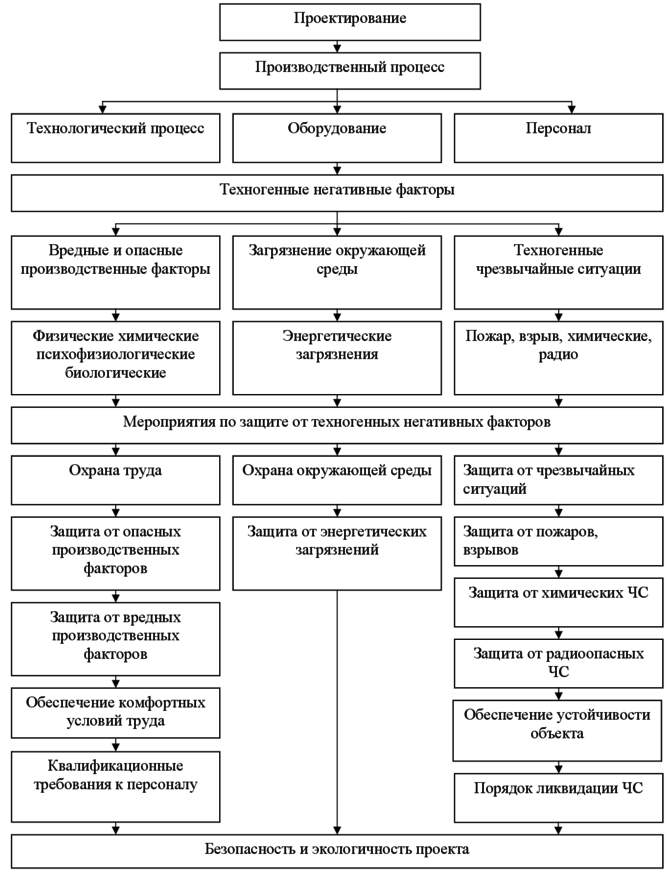
\includegraphics[width=0.85\textwidth]{diagrams/safety.png}
  \caption{Принципиальная блок-схема обеспечения безопасности объекта проектирования}
  \label{fig:safety}
\end{figure}

\subsection{Электромагнитное излучение}
Электромагнитным полем называется особая форма материи, посредством которой осуществляется взаимодействие между электрически заряженными частицами.

Токоведущие части действующих установок являются источником электромагнитных полей промышленной частоты.
Длительное действие электромагнитного поля на организм вызывает нарушение функционального состояния центральной нервной системы, сердечно-сосудистой системы, что приводит к быстрому утомлению, уменьшению работоспособности, болям в области сердца, изменению кровяного давления.

Параметрами степени воздействия электромагнитных полей на человека являются:
\begin{itemize}
  \item{интенсивность излучения;}
  \item{режим излучения;}
  \item{длина волны;}
  \item{размер облучаемой поверхности тела;}
  \item{особенности облучаемого организма;}
  \item{продолжительность воздействия.}
\end{itemize}

Для пользователя ПЭВМ основным источником электромагнитных полей и ионизирующих излучений является электронно-лучевая трубка дисплея.

Электромагнитные поля оказывают тепловое воздействие на организм, приводящее к структурным и функциональным изменениям в нем.

Воздействие электромагнитных полей способно вызвать изменение клеток и состава крови, замутнение хрусталика глаза, выпадение волос, ломку ногтей, ожоги, кожные заболевания и др.

Временно допустимые уровни электромагнитного потока на рабочем месте не должны превышать (для диапазона частот 5 Гц~--- 2 кГц):
\begin{itemize}
  \item{плотность магнитного потока~--- не более 250 нТл (по данным СанПиН 2.2.2./2.4.1340-03);}
  \item{напряженность электрического поля~--- не более 25 В/м;}
  \item{радиационное излучение на расстоянии 5 см от экрана~--- не более 100мкР/ч. (по данным СанПиН 2.2.2./2.4.1340-03).}
\end{itemize}

Электромагнитные поля радиочастот делятся на высокие частоты (ВЧ), ультравысокие частоты (УВЧ), сверхвысокие частоты (СВЧ).

На пользователя, работающего за монитором с ЭЛТ-дисплеем, воздействует практически весь диапазон излучений, оказывая биологическое и тепловое воздействие.

Во всех случаях предельно допустимое значение плотности потока энергии не должно превышать 10 мкВт/$\fc{см}^2$.

Однако, в настоящее время мониторы с ЭЛТ почти повсеместно вышли из употребления, будучи заменены на более безопасные мониторы с ЖК-дисплеем.
Эти мониторы характеризуются нулевым уровнем ионизирующих излучений, однако, тем не менее, создают повышенную нагрузку на ЦНС человека за счет нагрузки на зрительную систему.


\subsubsection{Электрический ток}

Действие электрического тока на органы человека может быть тепловым (ожог), механическим (разрыв тканей), химическим (электролиз) и биологическим (сокращение мышц, паралич дыхания и сердца).

При воздействии электрического тока на органы человека могут быть два вида поражения: электрические удары и электрические травмы.

Электрические удары~--- это возбуждение живых тканей организма протекающим через него электрическим током, проявляющееся в непроизвольных судорожных сокращениях различных мышц тела.
Они разделяются условно на четыре группы:
\begin{enumerate}
  \item{судорожное сокращение мышц без потери сознания;}
  \item{судорожное сокращение мышц с потерей сознания;}
  \item{потеря сознания и нарушение сердечной деятельности или дыхания;}
  \item{клиническая смерть, т.е. отсутствие дыхания и кровообращения.}
\end{enumerate}

По степени опасности поражения людей током рабочее пространство, оборудование дисплеями, относится к классу помещений без повышенной опасности согласно ПУЭ.

Основное питание в помещении должно осуществляется от трехфазной цепи током с частотой 50 Гц и напряжением 220 В.
Сеть трехфазная с заземленной нейтралью ГОСТ 12.1.030-81.

В соответствии с ГОСТ 12.1.030-81, в помещениях с электрооборудованием должна быть проложена шина защитного заземления (заземляющий проводник сечением не менее 120 мм), который должен металлически соединяться с заземляющей нейтралью электроустановок, от которой осуществляется электропитание оборудования.
Сопротивление заземляющего устройства, с которым соединяется нейтраль, должно быть не более 4 Ом.

Шина защитного заземления должна быть доступна для осмотра.

В соответствии с ГОСТ 12.1.030-81 подводка питания к дисплеям и устройствам должна осуществляться под съемным полом или в каналах.
Согласно ГОСТ 12.1.030-81, электрооборудование помещения относится к 1 классу защиты от поражения электрическим током, т.е. имеется рабочая изоляция, элемент для заземления и провод без зануляющей шины для подсоединения к источнику питания.

Для защиты персонала от попадания под опасное напряжение при неисправной изоляции необходимо предусмотреть защитное заземление, выполняемое в соответствии с ГОСТ 12.1.03-81.

Предупреждение коротких замыканий в электрической сети обеспечивается правильным выбором проводов (выбор сечения, токоведущих шин, марки проводов, видов изоляции); профилактические осмотры, ремонты.
Для быстрого отключения при коротком замыкании в комнате используются плавкие предохранители.

В случае аварийных ситуаций предусмотрено защитное отключение ПЭВМ за счет превращения тока замыкания на корпус в ток однофазного короткого замыкания с последующим срабатыванием защиты.

В рассматриваемом помещении установка всего электрооборудования выполнена в соответствии с нормами электробезопасности.
Питание осуществляется от трехфазной цепи с заземленной нетралью током с частотой 50 Гц и напряжением 220 В.

Электроснабжение всех потребителей осуществляется через главный распределительный щит.
Разводка электропитания по потребителям энергии осуществляется с помощью установленных в помещениях распределительных щитов и розеток.

Для отключения питания электрической сети в помещениях предусматриваются рубильники.

То есть, такой фактор как электробезопасность рассмотренной работы, а именно работа с персональным компьютером согласно ГОСТ 12.1.030-81 можно отнести по степени опасности к допустимым условиям труда.
В общем электробезопасность удовлетворяет ГОСТ 12.1.030-81 и дополнительных мер по защите не требуется.

\subsubsection{Требования по обеспечению пожарной безопасности}

Противопожарная защита имеет целью поиска самых экономически целесообразных и технически обоснованных способов и средств предупреждения пожаров и их ликвидации с минимальным ущербом при оптимальном использовании сил и технических средств тушения.

Пожарная безопасность~--- это состояние объекта, при котором исключается возможность пожара, а в случае его возникновения используются необходимые меры по устранению негативного влияния опасных факторов пожара на людей, сооружения и материальных ценностей.

Пожарная безопасность может быть обеспечена мерами пожарной профилактики и активной пожарной защиты.
Пожарная профилактика включает комплекс мероприятий, направленных на предупреждение пожара или уменьшение его последствий.

Активная пожарная защита~--- меры, обеспечивающие успешную борьбу с пожарами или взрывоопасной ситуацией.

В помещениях запрещается:
\begin{itemize}
  \item зажигать огонь;
  \item включать электрооборудование, если в помещении пахнет газом;
  \item курить;
  \item сушить что-либо на отопительных приборах;
  \item закрывать вентиляционные отверстия в электроаппаратуре.
\end{itemize}

Источниками воспламенения являются:
\begin{itemize}
  \item искра при разряде статического электричества;
  \item искры от электрооборудования;
  \item искры от удара и трения;
  \item открытое пламя.
\end{itemize}

При возникновении пожароопасной ситуации или пожара персонал должен немедленно принять необходимые меры для его ликвидации, одновременно оповестить о пожаре администрацию.

По взрывопожарной и пожарной опасности помещения делятся по категориям А, Б, В, Г, Д (в зависимости от свойств применяемых веществ и материалов). Исследуемое  помещение относится к категории В (помещение содержит горючие и трудногорючие жидкости, твердые горючие и трудногорючие вещества в малом количестве и материалы, способные только гореть при взаимодействии с кислородом воздуха).

В зависимости от пределов огнестойкости строительных конструкций установлены восемь степеней огнестойкости зданий: I, II, III, IIIа, IIIб, IV, IVа, V. Учитывая высокую стоимость оборудования, а также категорию пожароопасности, здание, в котором предусмотрено размещение ПЭВМ, должно быть отнесено к I или II степени огнестойкости согласно ГОСТ 12.1.004-89. По классификации класс пожароопасных зон относится к II-2-А (зона в которой обращаются твердые горючие вещества) согласно ПУЭ.

К горючим материалам, присутствующим в исследуемом помещении относятся: строительные материалы для акустической и эстетической отделки, двери, полы, изоляции силовых, сигнальных кабелей, обмотки радиотехнических деталей, изоляции соединительных кабелей, ячеек, блоков, панелей, жидкости для очистки элементов, узлов ПЭВМ от загрязнения и другие.

В качестве средств пожаротушения предусмотрены: огнетушитель и система автоматической пожарной сигнализации.

Работа с персональным компьютером удовлетворяет ГОСТ 12.1.004-89 в вопросах пожароопасности и взрывоопасности, следовательно, специализированнх дополнительных мер по защите не требуется.

\subsubsection{Психофизиологический фактор}
Работа оператора ЭВМ сопряжена с рядом физиологических неудобств~--- она ведется сидя, положение тела в течение рабочего дня меняется незначительно.
Хотя физическая нагрузка невелика, монотонность труда, повышенная нагрузка на зрительную систему и активная умственная работа ведут к высокой утомляемости.

Для обеспечения комфортного процесса работы оператор ЭВМ должен совершать регулярные перерывы в работе~--- раз в час необходимо на некоторое время дать отдых глазам и выполнить ряд простых физических упражнений, способствующих восстановлению тонуса организма.

Рабочее место~--- зона, оснащенная необходимыми техническими средствами, в которой совершается трудовая деятельность исполнителя или группы исполнителей, совместно выполняющих одну работу.

Под техническими средствами понимается основное и вспомогательное оборудование, устройства техники безопасности, санитарно гигиенические, культурно-бытовые устройства, необходимые для наиболее экономичного или наиболее производственного выполнения определенных технологических операций.

Под организацией рабочего места понимается система мероприятий по оснащения рабочего места средствами и предметами труда и их размещению в определенном порядке.

Как правило, оператор ПЭВМ не имеет возможности выбирать помещение или делать кардинальные перестановки оборудования для обеспечения наиболее оптимальных условий работы.
Поэтому рекомендации данной главы следует рассматривать как исходный материал или руководство к действию для организаторов работ с использованием ПЭВМ.
Они могут быть использованы операторами, заинтересованными в усовершенствовании своих рабочих мест.
Все приведенные требования включены в нормативный документ Госкомсанэпиднадзора <<Гигиенические требования к ПЭВМ и организации работы. Санитарные правила и нормы>>, вступивший в силу в июне 2003 г. (СанПин 2.2.2/2.4.1340-03).

В производственных помещениях, в которых работа с использованием ПЭВМ является вспомогательной, температура, относительная влажность и скорость движения воздуха на рабочих местах должны соответствовать действующим санитарным нормам микроклимата производственных помещений.
В соответствии с СанПиН 2.2.4.548-96 <<Гигиенические требования к микроклимату производственных помещений>>, для категории работ 1а оптимальные показатели таковы:
\begin{enumerate}
  \item В холодное время года:
  \begin{itemize}[leftmargin=*]
    \item температура воздуха: 22-24 $^{\circ}$C;
    \item относительная влажность: 40-60\%;
    \item скорость движения воздуха: 0,1 м/с.
  \end{itemize}
  \item В теплое время года:
  \begin{itemize}[leftmargin=*]
    \item температура воздуха: 23-25 $^{\circ}$C;
    \item относительная влажность: 40-60\%;
    \item скорость движения воздуха: 0,1 м/с.
  \end{itemize}
\end{enumerate}

Планировка рабочего места должна удовлетворять требованиям удобства работы и экономии энергии и времени оператора, соблюдения правил личной и производственной безопасности:
\begin{itemize}
  \item При размещении рабочих мест с ПЭВМ расстояние между рабочими столами с видеомониторами (в направлении тыла поверхности одного видеомонитора и экрана другого видеомонитора), должно быть не менее 2,0 м, а расстояние между боковыми поверхностями видеомониторов~--- не менее 1,2м.
  \item Рабочие места с ПЭВМ при выполнении творческой работы, требующей значительного умственного напряжения или высокой концентрации внимания, рекомендуется изолировать друг от друга перегородками высотой 1,5-2,0 м.
  \item Рабочие места с ПЭВМ в помещениях с источниками вредных производственных факторов должны размещаться в изолированных кабинах с организованным воздухообменом.
  \item Конструкция рабочего стола должна обеспечивать оптимальное размещение на рабочей поверхности используемого оборудования с учетом его количества и конструктивных особенностей, характера выполняемой работы. При этом допускается использование рабочих столов различных конструкций, отвечающих современным требованиям эргономики.
  \item Конструкция рабочего стула (кресла) должна обеспечивать поддержание рациональной рабочей позы при работе на ПЭВМ, позволять изменять позу с целью снижения статического напряжения мышц шейно-плечевой области и спины для предупреждения развития утомления. Тип рабочего стула (кресла) следует выбирать с учетом роста пользователя, характера и продолжительности работы с ПЭВМ.
  \item Рабочий стул (кресло) должен быть подъемно-поворотным, регулируемым по высоте и углам наклона сиденья и спинки, а также расстоянию спинки от переднего края сиденья, при этом регулировка каждого параметра должна быть независимой, легко осуществляемой и иметь надежную фиксацию.
  \item Поверхность сиденья, спинки и других элементов стула (кресла) должна быть полумягкой, с нескользящим, слабо электризующимся и воздухопроницаемым покрытием, обеспечивающим легкую очистку от загрязнений.
  \item Экран видеомонитора должен находиться от глаз пользователя на расстоянии 600 -- 700 мм, но не ближе 500 мм с учетом размеров алфавитно-цифровых знаков и символов.
\end{itemize}

\subsubsection{Требования к персоналу, эксплуатирующему средства вычислительной техники}
К самостоятельной эксплуатации электроаппаратуры допускается только специально обученный персонал не моложе 18 лет, пригодный по состоянию здоровья и квалификации к выполнению указанных работ.

Перед допуском к работе персонал должен пройти вводный и первичный инструктаж по технике безопасности с показом безопасных и рациональных примеров работы. Затем не реже одного раза в 6 месяцев проводится повторный инструктаж, возможно, с группой сотрудников одинаковой профессии в составе не более 20 человек. Внеплановый инструктаж проводится при изменении правил по охране труда, при обнаружении нарушений персоналом инструкции по технике безопасности, изменении характера работы персонала.

В помещениях, в которых постоянно эксплуатируется электрооборудование должны быть вывешены в доступном для персонала месте инструкции по технике безопасности, в которых также должны быть определены действия персонала в случае возникновения аварий, пожаров, электротравм.

Руководители структурных подразделений несут ответственность за организацию правильной и безопасной эксплуатации средств вычислительной техники и периферийного оборудования, эффективность их использования; осуществляют контроль за выполнением персоналом требований настоящей инструкции по технике безопасности.

\subsubsection{Расчет освещенности}
Профессиональным заболеванием операторов и программистов является ухудшение зрения.
Так как параметры помещения, в котором ведется работа, и используемой техники (персональной ПЭВМ) удовлетворяют санитарным нормам, то особое внимание следует уделить освещенности рабочего места.

Расчет освещенности проводится с путем расчета коэффициента использования с использованием метода светового потока).
Он позволяет учесть прямую и отраженную составляющую светового потока от потолка, стен и рабочих поверхностей.

Имеются следующие исходные данные:
\begin{itemize}
  \item площадь помещения~--- 2,5x4 м;
  \item высота подвеса светильников $h_\fc{св}$= 2,5 м;
  \item источник освещения~--- лампа люминесцентная (ЛБА), яркость фона~--- светлая;
  \item яркость объекта~--- средняя;
  \item система освещения~--- общая;
  \item коэффициент отражения побеленного потолка: $p_\fc{п}$= 0,7;
  \item коэффициент отражения стен, обклеенных обоями: $p_c$ = 0,5;
  \item коэффициент отражения расчетной поверхности: $p_p$ = 0,3.
\end{itemize}

По таблице <<Нормы освещенности при искусственном освещении и коэффициент естественного освещения (для 3 пояса светового климата РФ) при естественном и совмещенном освещении>> (СНиП 23-05-95), исходя из характеристик зрительной работы определяем разряд и подразряд зрительной работы как IV-В.
Данному разряду соответствует норма искусственного освещения при системе комбинированного освещения 300 лк.

Норма рабочего искусственного освещения составляет $E_\fc{он}$ = 400 лк. Коэффициент запаса равен $K_3$ = 1,5, высота подвеса светильников $h_\fc{св}$ = 2,2 м.

Определяем индекс помещения:

$i = {{a \cdot b} \over {(a + b) \cdot h_\fc{св}}} = {{2,5 \cdot 4} \over {(2,5 + 4) \cdot 2.5}} {\approx 0,6}$

Тип лампы~--- ЛБА, люминесцентная белого света, амальгамная.
Интерполированием находим коэффициент использования: $\eta$ = 0,52.

Определяем расстояние между светильниками и по нему~--- число светильников в помещении.
Рекомендованное отношение $\lambda = {I_\fc{св} \over h_\fc{св}}$ равно 0,8--1,2. Принимаем $\lambda$ = 0,8, тогда  $I_\fc{св} = 0,8 \cdot 2,5 = 2$ м.

Число светильников при размещении по углам квадрата вычисляется по формуле:

$n = {{a \cdot b} \over {I_\fc{св}^2}} = {{2,5 \cdot 4} \over {4}} \approx 3$

Определяем световой поток одной лампы.
Коэффициент минимальной освещенности, зависящий от размещения и светораспределения светильников, создающих некоторую неравномерность распределения светового потока по расчетной плоскости, принимаем равным $Z$ = 1,1.

$\Phi_o = {{E \cdot S \cdot Z \cdot K_3} \over {n \cdot \eta}} = {{400 \cdot 10 \cdot 1,1 \cdot 1,5} \over {3 \cdot 0,52}} \approx 4231 (\fc{лм})$

Выбираем лампу ЛБ-80-7 со световым потоком 5200 лм, срок продолжительности горения 12000 час, мощность 80 Вт.
Суммарная мощность осветительной установки общего освещения:

$P = P_o \cdot n = 80 \cdot 3 = 240 (\fc{Вт})$

Таким образом, на площадь 2,5 x 4 м для работы за дисплеем при общем освещении должны использоваться 3 светильника по 1 лампе ЛБА-80-7.


\subsection{Защита окружающей среды}

\subsubsection{Анализ воздействия компьютера на окружающую среду}
В жизненном цикле компьютерной техники можно выделить три этапа: производство, эксплуатация, утилизация.

Вопросы защиты окружающей среды в процессе производства компьютеров возникли давно и регламентируются сейчас, в частности стандартом ТСО-03 NUTEC, по которому контролируются выбросы токсичных веществ, условия работы и др.
Согласно ТСО-03 произведенное оборудование может быть сертифицировано лишь в том случае, если не только контролируемые параметры самого оборудования соответствуют требованиям этого стандарта, но и технология производства этого оборудования отвечает требованиям стандарта.

Воздействие компьютеров на окружающую среду при эксплуатации регламентировано рядом стандартов.
Выделяют две группы стандартов и рекомендаций: по безопасности и эргономике.

При утилизации старых компьютеров происходит их разработка на фракции: металлы, пластмассы, стекло, провода, штекеры.
Из одной тонны компьютерного лома получают до 200 кг меди, 480 кг железа и нержавеющей стали, 32 кг алюминия, 3 кг серебра, 1 кг золота и 300 г палладия.

Переработку промышленных отходов производят на специальных полигонах, создаваемых в соответствии с требованиями СНиП 2.01.28-85 и предназначенных для централизованного сбора обезвреживания и захоронения токсичных отходов промышленных предприятий, НИИ и учреждений.

\subsubsection{Влияние электромагнитных излучений компьютера на здоровье человека}
По обобщенным данным, у работающих за монитором от 2 до 6 часов в сутки функциональные нарушения центральной нервной системы происходят в среднем в 4,6 раза чаще, чем в контрольных группах, болезни сердечнососудистой системы~--- в 2 раза чаще, болезни верхних дыхательных путей~--- в 1,9 раза чаще, болезни опорно-двигательного аппарата--- в 3,1 раза чаще.
С увеличением продолжительности работы на компьютере соотношения здоровых и больных среди пользователей резко возрастает.

Глобальная информатизация и, как следствие, широкое применение компьютерной техники в современной жизни привели к необходимости контролировать эргономические параметры используемых компьютеров.
В большинстве развитых стран мирового сообщества существуют стандарты, регламентирующие допустимые параметры излучения компьютерной техники.

Вредоносность некоторых диапазонов излучений, генерируемых компьютерами, подтверждается медицинскими исследованиями.
Экспериментальные данные говорят о том, что длительное воздействие электромагнитных волн приводит к нарушениям деятельности центральной нервной, гормональной и сердечно-сосудистой систем, изменению биохимических показателей крови.
Субъективные ощущения человека, систематически подвергающегося облучению, проявляются в виде симптомов частой головной боли, утомляемости, ухудшения памяти, болевых ощущений в области сердца, желудка и других внутренних органов.

Основным источником неблагоприятного воздействия компьютера на здоровье пользователя являются мониторы на основе электронно-лучевой трубки.
Однако не стоит недооценивать и излучения, связанные с работой системного блока, источников бесперебойного питания и прочих устройств.
Все эти элементы формируют сложную электромагнитную обстановку на рабочем месте пользователя ЭВМ.

К основным факторам неблагоприятного воздействия работы с компьютером можно отнести следующие:
\begin{itemize}
  \item электромагнитное поле сложного спектрального состава в широком диапазоне частот (от 10 Гц до 1000 МГц);
  \item электростатический заряд на ЭЛТ монитора;
  \item ультрафиолетовое, инфракрасное и рентгеновское излучения;
  \item эргономические параметры экрана (блики, мерцание, контрастность).
\end{itemize}

На биологическую реакцию человека влияют такие параметры электромагнитных полей ЭВМ, как интенсивность и частота излучения, продолжительность облучения и модуляция сигнала, частотный спектр и периодичность действия.
Сочетание вышеперечисленных параметров может давать различные последствия для реакции облучаемого биологического объекта.
Кроме того, следует отметить и такие дополнительные факторы, характерные для пользователей ПЭВМ, как изменение аэроионного состава воздуха, увеличение нагрузки на зрение, стрессовые факторы, синдром длительной статической нагрузки и пр.

В настоящее время существует достаточно данных, указывающих на отрицательное влияние работы с компьютером на все жизненно важные системы человека.
Кроме того, биологический эффект электромагнитных полей в условиях длительного воздействия может, накапливаясь, стать причиной тяжелых заболеваний.

В качестве технических стандартов безопасности мониторов широко известны шведские ТСО-92, 95, 99, 03 и МРR-II.
Они ограничивают параметры излучения монитора, потребления электроэнергии, визуальные параметры.

В части электромагнитных полей стандарту МРR-II соответствуют российские санитарные нормы СанПиН 2.2.2006-05 <<Руководство по гигиенической оценке факторов рабочей среды и трудовых процессов. Критерии и классификация условий труда>>.

\subsubsection{Мероприятия по защите окружающей среды}
Для охраны окружающей среды необходимо разработать и освоить оптимальную технологию утилизации устаревших или пришедших в негодность внутренних заменяемых компонентов компьютера (интегральных схем, плат, микроконтроллеров, механических частей компьютера, шлейфов и т. д.), а также внешних магнитных носителей.
Для этого на первом этапе утилизации необходимо сортировать и складировать в отдельные контейнеры по типу~--- отдельно провода, платы, механизмы, бумагу.
На втором этапе нужно отделять от неработающих деталей исправные части и использовать их в качестве запчастей для работающих изделий (если это возможно).
Оставшиеся~--- сдавать в соответствующие профильные ремонтные или утилизирующие организации.


\subsection{Защита в чрезвычайных ситуациях}

\subsubsection{Причины возможных чрезвычайных ситуаций}
Чрезвычайная ситуация~--- внешне неожиданная, внезапно возникающая обстановка, которая характеризуется резким нарушением установившегося процесса, оказывающая значительное отрицательное влияние на жизнедеятельность людей, функционирование экономики, социальную сферу и окружающую среду.

В г. Ульяновске могут возникнуть чрезвычайные ситуации производственного (техногенного) и природного характера.

Чрезвычайные ситуации производственного характера:
\begin{itemize}
  \item транспортная авария (катастрофа);
  \item пожары, взрывы, с последующим горением;
  \item аварии с выбросом вредных веществ;
  \item обрушение сооружений;
  \item аварии на коммунальных системах жизнеобеспечения;
  \item аварии на электроэнергетических системах.
\end{itemize}

В этих ситуациях источниками опасности будут являться автотранспорт и железнодорожный транспорт, предприятия, в производстве которых применяются вредные вещества.

Источниками опасности являются также газопровод, автозаправочные станции, на которых сосредоточена большая емкость бензина и дизельного топлива, НИИАР в г. Димитровграде.

Чрезвычайные ситуации природного происхождения:
\begin{itemize}
  \item опасные метеорологические явления (бури, град, сильный ливень, мороз, метель, гололед, сильная жара и др.);
  \item инфекционная загрязненность р. Волги.
  \item повышение предельно допустимых концентраций вредных примесей в атмосфере;
  \item образование обширной зоны кислотных осадков.
\end{itemize}

Необходимо отметить, что ЧС природного происхождения почти не имеют влияния на работу комплекса ПЭВМ, а в основном на персонал.
Последнее происходит в случае плохой конструкции зданий, в которых расположены производственные помещения и офисы.

Работе самого комплекса ПЭВМ существенно могут помешать ЧС техногенного характера.
Возникновение ЧС этой группы может привести следующему:
\begin{itemize}
  \item физическое повреждение ПЭВМ, его частичное или полное разрушение в результате пожара, взрыва, обрушения сооружений;
  \item отключение электроэнергии от комплекса ПЭВМ в результате аварии на станции энергоснабжения;
  \item сбой в работе программы, частичная или полная потеря информации, повреждение поверхности магнитных носителей в результате воздействия электромагнитных импульсов большой мощности.
\end{itemize}

\subsubsection{Мероприятия по предотвращению чрезвычайных ситуаций}
Во избежание возникновения ЧС первой подгруппы персоналу необходимо соблюдать правила электро- и пожарной безопасности, а также регулярно проходить инструктаж по технике безопасности.

Для того чтобы избежать последствий ЧС второй подгруппы, рекомендуется использовать бесперебойный источник питания. Это позволит сохранить и закончить работу в нормальном режиме без потери какой-либо информации.

Для частичного избежания последствий ЧС третьей подгруппы можно использовать оптические носители информации, которые не подвержены воздействию электромагнитных импульсов.
При этом рекомендуется периодически делать копии необходимой информации при высокой вероятности возникновения ЧС, приводящих к последствиям третьей группы.

\subsubsection{Аппаратные средства защиты}

Под аппаратными средствами защиты понимаются специальные средства, непосредственно входящие в состав технического обеспечения и выполняющие функции защиты как самостоятельно, так и в комплексе с другими средствами, например с программными.
Можно выделить некоторые наиболее важные элементы аппаратной защиты:
\begin{itemize}
  \item защита от сбоев в электропитании;
  \item защита от сбоев серверов, рабочих станций и локальных компьютеров;
  \item защита от сбоев устройств для хранения информации;
  \item защита от электромагнитных излучений.
\end{itemize}


\subsubsection{Мероприятия по обеспечению пожарной безопасности и расчет средств пожаротушения}

При определении видов и количества первичных средств пожаротушения следует учитывать физико-химические и пожароопасные свойства горю чих веществ, их отношение к огнетушащим веществам, а также площадь производственных помещений.

Комплектование технологического оборудования огнетушителями осуществляется согласно требованиям технических условий на это оборудование или соответствующим правилам пожарной безопасности.

Выбор типа и расчет необходимого количества огнетушителей в защищаемом помещении или на объекте следует проводить в зависимости от их огнетушащей способности, предельной площади, а также класса пожара горючих веществ и материалов:
\begin{itemize}
  \item класс А~--- пожары твердых веществ, в основном органического происхождения, горение которых сопровождается тлением (древесина, текстиль, бумага);
  \item класс В~--- пожары горючих жидкостей или плавящихся твердых веществ;
  \item класс С~--- пожары газов;
  \item класс D~--- пожары металлов и их сплавов;
  \item класс Е~--- пожары, связанные с горением электроустановок.
\end{itemize}

Выбор типа огнетушителя (передвижной или ручной) обусловлен размерами возможных очагов пожара.
При их значительных размерах необходимо использовать передвижные огнетушители.

В соответствии с НПБ 105-03 помещение относится к категории В (помещение содержит горючие и трудногорючие жидкости, твердые горючие и трудногорючие вещества в малом количестве и материалы, способные только гореть при взаимодействии с кислородом воздуха).
По нормам оснащения помещений ручными огнетушителями в помещениях категории В, при возможности пожара класса А, необходимо установить 2 пенных и водных огнетушителя вместимостью 10 л или 2 порошковых огнетушителя вместимостью 5 л.
Необходимости оборудования пожарного щита в помещении нет.

Меры противопожарной безопасности:

\begin{enumerate}
\item Желательно установить на рабочем месте пожарную сигнализацию (дымоулавливатели).
\item Для борьбы с возможными пожарами класса А возможна установка пожарного щита типа ЩП-А.
  Для помещения типа Д предельная площадь покрываемая одним пожарным щитом равна 1800 м.
\end{enumerate}

В комплектацию пожарного щита типа ЩП-А входят:
\begin{itemize}
  \item огнетушители пенные и водные вместимостью 10 л~--- 2 шт.;
  \item огнетушители порошковые вместимостью 10 л~--- 1 шт.;
  \item лом~--- 1 шт.;
  \item багор~--- 1 шт.;
  \item ведро~--- 2 шт.;
  \item лопата штыковая~--- 1 шт.;
  \item лопата совковая~--- 1 шт.
\end{itemize}

\subsection{Выводы по разделу}
В данном разделе был произведен анализ основных вредных и опасных факторов исследуемого объекта.
По результатам анализа были разработаны мероприятия по обеспечению безопасных и комфортных условияй труда оператора ЭВМ.

Для проверки соответствия рабочий условий нормативным был произведен расчет освещенности.

Были разработаны мероприятия по охране окружающей среды и противостоянию возможным чрезвычайным ситуациям.

В пункте \ref{sec:safety:data} указано, что класс условий труда~--- 3.2, вредный.
Вредность работы оператора ЭВМ объясняется следующими факторами: высокая напряженность интеллектуального труда, творческий характер работы, потребность в постоянном сосредоточении внимания, работа в условиях высокого уровня шума, производимого ЭВМ, физическая монотонность выполняемых операций (набор текста на клавиатуре).

Таким образом, на основании выше изложенного, при условии выполнения всех мероприятий, соблюдения норм трудовой дисциплины и распорядка дня, рабочее место и рабочий процесс оператора персональной ЭВМ являются вредными, но не травмоопасными.